\input{EDAN20_header}


\subtitle{Chapter 17: Transformers: Encoder-Decoder and Decoder\\
\footnotesize{
\url{https://link.springer.com/chapter/10.1007/978-3-031-57549-5_17}
}}
\date{October 9, 2025}

%\AtBeginSection[]
%{
%   \begin{frame}
%       \frametitle{Outline}
%       \tableofcontents[currentsection]
%   \end{frame}
%}


\begin{document}
\frame{\titlepage
}

%\section<presentation>*{Outline}
%\begin{frame}
%  \frametitle{Outline}
%  \tableofcontents[part=1,pausesections]
%\end{frame}
%
%
%\AtBeginSubsection[]
%{
%  \begin{frame}<beamer>
%    \frametitle{Outline}
%    \tableofcontents[current,currentsubsection]
%  \end{frame}
%}

\section{Language Technology}
\subsection{Chapter 17: Transformers: Encoder-Decoder and Decoder}

\begin{frame}[fragile]
\frametitle{Machine Translation}\color{structure}
Process of translating automatically a text from a source language into a target language\\
Started after the 2nd world war to translate documents from Russian to English\\
Early working systems from French to English in Canada\\
Renewed huge interest with the advent of the web\\
Google claims it has more than 500m users daily worldwide, with 103 languages.\\
Massive progress permitted by the encoder-decoder networks
\end{frame}

\begin{frame}[fragile]
\frametitle{Corpora for Machine Translation}\color{structure}
Initial ideas in machine translation: use bilingual dictionaries and formalize grammatical rules to transfer them from a source language to a target language.\\
Statistical machine translation:
\begin{enumerate}\color{structure}
\item Use very large bilingual corpora;
\item Align the sentences or phrases, and
\item Given a sentence in the source language, find the matching sentence in the target language.
\end{enumerate} 
Pioneered at IBM on French and English with Bayesian statistics.\\
As of today, the encoder-decoder architecture is dominant
\end{frame}

\begin{frame}[fragile]
\frametitle{Parallel Corpora (Swiss Federal Law)}
\color{structure}
\begin{small}
\begin{center}
\begin{tabular}{p{105pt}p{105pt}p{105pt}}
\hline
\textbf{German}& \textbf{French}& \textbf{Italian} \\
\hline
\textbf{Art. 35 Milchtransport}& \textbf{Art. 35 Transport du lait}& \textbf{Art. 35 Trasporto del latte} \\
\hline
1 Die Milch ist schonend und hygienisch in den Verarbeitungsbetrieb zu transportieren. Das Transportfahrzeug ist stets sauber zu halten. Zusammen mit der Milch d\"{u}rfen keine Tiere und milchfremde Gegenst\"{a}nde transportiert werden, welche die Qualit\"{a}t der Milch beeintr\"{a}chtigen k\"{o}nnen. &
1 Le lait doit \^{e}tre transport\'{e} jusqu'\`{a} l'entreprise de transformation avec m\'{e}nagement et conform\'{e}ment aux normes d'hygi\`{e}ne. Le v\'{e}hicule de transport doit \^{e}tre toujours propre. Il ne doit transporter avec le lait aucun animal ou objet susceptible d'en alt\'{e}rer la qualit\'{e}.
&
1 Il latte va trasportato verso l'azienda di trasformazione in modo accurato e igienico. Il veicolo adibito al trasporto va mantenuto pulito. Con il latte non possono essere trasportati animali e oggetti estranei, che potrebbero pregiudicarne la qualit\`{a}.\\
 &&\\
2 Wird Milch ausserhalb des Hofes zum Abtransport bereitgestellt, so ist sie zu beaufsichtigen. &
2 Si le lait destin\'{e} \`{a} \^{e}tre transport\'{e} est d\'{e}pos\'{e} hors de la ferme, il doit \^{e}tre plac\'{e} sous surveillance.
&
 2 Se viene collocato fuori dall'azienda in vista del trasporto, il latte deve essere sorvegliato.\\
&&\\
3 Milchpipelines sind nach den Anweisungen des Herstellers zu reinigen und zu unterhalten.
&
3 Les lactoducs des exploitations d'estivage doivent \^{e}tre nettoy\'{e}s et entretenus conform\'{e}ment aux instructions du fabricant.
&
3 I lattodotti vanno puliti e sottoposti a manutenzione secondo le indicazioni del fabbricante. \\
\hline
\end{tabular}
\end{center}
\end{small}
\end{frame}

\begin{frame}[fragile]
\frametitle{Alignment (Brown et al. 1993)}
\color{structure}
Canadian Hansard
 
\begin{center}
\input{\livreimg/08posstat/posstat12.tikz}
\end{center}
\vspace{0.75cm}
\begin{center}
\input{\livreimg/08posstat/posstat13.tikz}
\end{center}
\end{frame}

\begin{frame}[fragile]
\frametitle{Transformers: The Encoder-Decoder}\color{structure}
Transformers were originally developed for machine translation\\
Initial language pairs were: English-French, English-German, and the reverse\\

\begin{figure}[tb]
\begin{center}
 \includegraphics[scale=1.]{\livreimg/07denserep/the-annotated-transformer_14_0.png}
\end{center}
\end{figure}
The input corresponds to words in the source language (say English) and the output in the target language (French or German)
\end{frame}


%\begin{frame}[fragile]
%\frametitle{Language Models}\color{structure}
%\begin{itemize}\color{structure}
%\item A language model is a statistical estimate of a word sequence.
%\item Originally developed for speech recognition\\
%\item A causal or autoregressive language model enables us to predict the next word given a sequence of previous words:\\
%\item Given the sequence $x_1, x_2, ..., x_{n-1}$, predict $x_n$
%\[
%P(x_n|x_1, x_2, ..., x_{n-1})
%\]
%\item We approximated sequences with:
%\begin{itemize}\color{structure}
%\item Bigrams, sequences of two words, given the previous word predict the next one
%\item $N$-grams, sequences of $N$ words
%\end{itemize}
%\item Evaluation with the negative log-likelihood:
%\[
%L(\mathbf{x}) = -\sum_i \log(x_i|x_{i-N}, x_{i - N + 1}, ..., x_{i-1};\theta)
%\]
%\end{itemize}
%\end{frame}

\begin{frame}[fragile]
\frametitle{Generation}\color{structure}
The transformer consists of  an encoder and a decoder.
\begin{enumerate}\color{structure}
\item The encoder builds a representation of an input sequence, $(x_1, x_2, ..., x_n)$ called the memory, $M$,
\[
\text{encoder}(x_1, x_2, ..., x_n) = M;
\]
\item The decoder uses $M$ and a start symbol \verb=<s>= as first input. The decoder generates a new output and concatenates it until it generates a stop symbol, \verb=</s>=:
\[
\begin{array}{rcl}
\text{decoder}(M, \texttt{<s>}) &= &y'_1,\\
\text{decoder}(M, \texttt{<s>}, y'_1) &=& y'_2,\\
\text{decoder}(M, \texttt{<s>}, y'_1, y'_2) & = & y'_3,\\
...\\
\text{decoder}(M, \texttt{<s>}, y'_1, y'_2, ..., y'_{p-1}) & = & y'_p,\\
\text{decoder}(M, \texttt{<s>}, y'_1, y'_2, ..., y'_{p-1}, y'_{p})& = & \texttt{</s>}.\\
\end{array}
\]
\end{enumerate}  
\end{frame}

\begin{frame}[fragile]
\frametitle{Example}\color{structure}
For two source and target sequences of characters in English and French:
\begin{verbatim}
Source: ('H', 'e', 'l', 'l, 'o')
Target: ('B', 'o', 'n', 'j', 'o', 'u', 'r')
 \end{verbatim}
 We first encode \textit{Hello}, the source sequence:
\[
\text{encoder}(H, e, l, l, o) = M;
\]
Using $M$ and  $\texttt{<s>}$, we decode the target sequence:
\[
\begin{array}{rcl}
\text{decoder}(M, \texttt{<s>}) & = &B,\\
\text{decoder}(M, \texttt{<s>}, B) & = &o,\\
...\\
\text{decoder}(M, \texttt{<s>}, B, o, n, j, o, u)& = &r,\\
\text{decoder}(M, \texttt{<s>}, B, o, n, j, o, u, r) & = &\texttt{</s>},\\
\end{array}
\]
 We would need a linear layer to map it to the character predictionn
\end{frame}

\begin{frame}[fragile]
\frametitle{Decoder (I)}\color{structure}
\begin{columns}
\begin{column}[c]{0.62\textwidth}
The right part of the initial transformer\\
Same components:
\begin{enumerate}\color{structure}
\item Attention
\item Add and norm
\item Feed-forward
\end{enumerate}
\end{column}
\begin{column}[c]{0.4\textwidth}
\begin{figure}[tb]
\begin{center}
 \includegraphics[scale=1.2]{\livreimg/07denserep/the-annotated-transformer_14_0.png}
\end{center}
\end{figure}
\end{column}
\end{columns}
\end{frame}

\begin{frame}[fragile]
\frametitle{Decoder (II)}\color{structure}
\begin{columns}
\begin{column}[c]{0.62\textwidth}

But: 
\begin{enumerate}\color{structure}
\item Two attentions: 
\begin{enumerate}\color{structure}
\item \textbf{Masked} self-attention on the inputs
\item \textbf{Cross-attention} with the encoded source
\end{enumerate}
\item Second attention module: $Q = {X}_\text{dec\_sublayer}$, $K = Y_\text{enc}$, $V = Y_\text{enc}$;
\item The decoder predicts the input shifted by one (linear and softmax)
\end{enumerate}
\end{column}
\begin{column}[c]{0.4\textwidth}
\begin{figure}[tb]
\begin{center}
 \includegraphics[scale=1.2]{\livreimg/07denserep/the-annotated-transformer_14_0.png}
\end{center}
\end{figure}
\end{column}
\end{columns}
\end{frame}

\begin{frame}[fragile]
\frametitle{Transformer Embeddings}\color{structure}
\begin{columns}
\begin{column}[c]{0.62\textwidth}

In Vaswani's paper, the input and output embeddings and the last linear module share the same matrix (weights)\\
Same with BERT in the pretraining step for the input embeddings and last linear layer.

See code: \url{https://github.com/google-research/bert/blob/master/run_pretraining.py#L240})
\end{column}
\begin{column}[c]{0.4\textwidth}
\begin{figure}[tb]
\begin{center}
 \includegraphics[scale=1.2]{\livreimg/07denserep/the-annotated-transformer_14_0.png}
\end{center}
\end{figure}
\end{column}
\end{columns}
\end{frame}



\begin{frame}[fragile]
\frametitle{Prediction with Characters}\color{structure}
Translation pairs: (Source sentence, Target sentence)\\
For instance: (Hello, Bonjour), here with characters
\begin{enumerate}\color{structure}
\item Encoder input: \textit{H e l l o} 
\item Decoder input: \textit{B o n j o u r} and the encoded \textit{H e l l o}
\item Decoder output: \textit{B o n j o u r} shifted by one to the left 
\item We align the decoder strings with \verb=<s>= and \verb=</s>=
\end{enumerate}
\begin{center}
\scalebox{0.8}{
\tikzset{every picture/.style={line width=0.75pt}} %set default line width to 0.75pt        

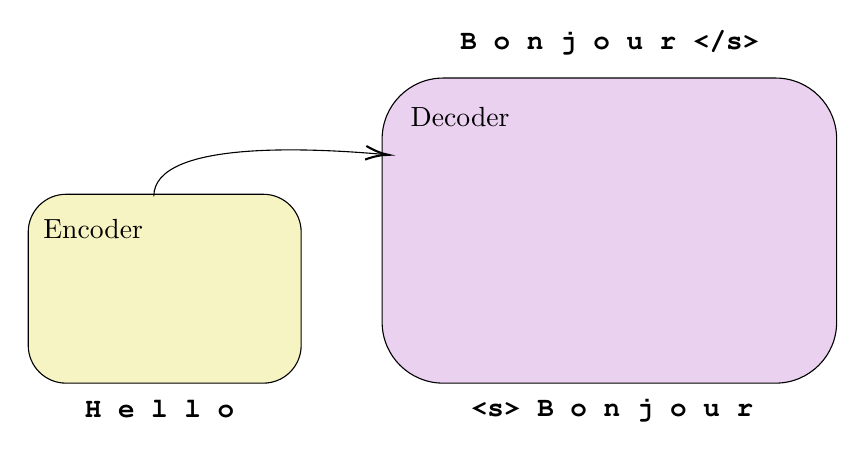
\begin{tikzpicture}[x=0.75pt,y=0.75pt,yscale=-1,xscale=1]
%uncomment if require: \path (0,404); %set diagram left start at 0, and has height of 404

%Rounded Rect [id:dp7267211892273574] 
\draw  [fill={rgb, 255:red, 243; green, 237; blue, 161 }  ,fill opacity=0.63 ] (186,115.2) .. controls (186,105.15) and (194.15,97) .. (204.2,97) -- (299.3,97) .. controls (309.35,97) and (317.5,105.15) .. (317.5,115.2) -- (317.5,169.8) .. controls (317.5,179.85) and (309.35,188) .. (299.3,188) -- (204.2,188) .. controls (194.15,188) and (186,179.85) .. (186,169.8) -- cycle ;
%Rounded Rect [id:dp2457933556767944] 
\draw  [fill={rgb, 255:red, 234; green, 209; blue, 239 }  ,fill opacity=1 ] (356.5,70.4) .. controls (356.5,54.16) and (369.66,41) .. (385.9,41) -- (546.1,41) .. controls (562.34,41) and (575.5,54.16) .. (575.5,70.4) -- (575.5,158.6) .. controls (575.5,174.84) and (562.34,188) .. (546.1,188) -- (385.9,188) .. controls (369.66,188) and (356.5,174.84) .. (356.5,158.6) -- cycle ;
%Curve Lines [id:da5049905334539878] 
\draw    (246.5,98) .. controls (246.5,70.42) and (324.6,74.86) .. (358.01,77.86) ;
\draw [shift={(359.5,78)}, rotate = 185.27] [color={rgb, 255:red, 0; green, 0; blue, 0 }  ][line width=0.75]    (10.93,-3.29) .. controls (6.95,-1.4) and (3.31,-0.3) .. (0,0) .. controls (3.31,0.3) and (6.95,1.4) .. (10.93,3.29)   ;

% Text Node
\draw (212,195) node [anchor=north west][inner sep=0.75pt]   [align=left] {{\fontfamily{pcr}\selectfont \textbf{H e l l o}}};
% Text Node
\draw (192,108) node [anchor=north west][inner sep=0.75pt]   [align=left] {Encoder};
% Text Node
\draw (398,194) node [anchor=north west][inner sep=0.75pt]   [align=left] {{\fontfamily{pcr}\selectfont \textbf{<s> B o n j o u r}}};
% Text Node
\draw (393,17) node [anchor=north west][inner sep=0.75pt]   [align=left] {{\fontfamily{pcr}\selectfont \textbf{B o n j o u r </s>}}};
% Text Node
\draw (369,54) node [anchor=north west][inner sep=0.75pt]   [align=left] {Decoder};
\end{tikzpicture}}
\end{center}
\end{frame}

\begin{frame}[fragile]
\frametitle{Training and Inference Steps}\color{structure}

\begin{enumerate}\color{structure}
\item Training step
%$\uparrow$
\begin{center}
\begin{tiny}
\begin{tabular}{rrlrcccccccccc}
\hline
&&&Target output:& B &o& n &j &o &u& r &</s>\\
&$\Rsh$&Encoded source:&$\longrightarrow$&$\uparrow$&$\uparrow$&$\uparrow$&$\uparrow$&$\uparrow$&$\uparrow$&$\uparrow$&$\uparrow$\\
Source input: &H e l l o&& Target input:&<s> &B& o& n& j& o& u& r \\
\hline
\end{tabular}
\end{tiny}
\end{center}
\item Inference:
\begin{center}
\begin{tiny}
\begin{tabular}{rrrrcccccccccc}
\hline
&&&Target output:& B &...\\
&$\Rsh$&Encoded source:&$\longrightarrow$&$\uparrow$&\\
Source input: &H e l l o&& Target input:&<s> &B& ...\\
\hline
\end{tabular}
\end{tiny}
\end{center}
\end{enumerate}
\end{frame}


\begin{frame}[fragile]
\frametitle{Vaswani's Attention Scores}\color{structure}
The attention scores are scaled and normalized by the softmax function.
\[
 \text{softmax}(\frac{{Q}  {K}^\intercal}{\sqrt{d_k}}),
\]

\begin{scriptsize}
\begin{tabular}{rrrrrrrrrrrr}
&i&must&go&back&to&my&ship&and&to&my&crew\\
i&0.36&0.05&0.07&0.05&0.04&0.19&0.01&0.02&0.04&0.19&0.01\\
must&0.14&0.20&0.10&0.06&0.11&0.10&0.03&0.05&0.11&0.10&0.02\\
go&0.18&0.09&0.14&0.09&0.08&0.13&0.02&0.04&0.08&0.13&0.02\\
back&0.14&0.05&0.09&0.19&0.08&0.12&0.03&0.06&0.08&0.12&0.03\\
to&0.11&0.11&0.09&0.09&0.15&0.08&0.04&0.07&0.15&0.08&0.03\\
my&0.19&0.03&0.05&0.04&0.03&0.29&0.01&0.02&0.03&0.29&0.01\\
ship&0.03&0.03&0.03&0.04&0.05&0.03&0.55&0.03&0.05&0.03&0.13\\
and&0.10&0.08&0.07&0.10&0.12&0.09&0.04&0.15&0.12&0.09&0.04\\
to&0.11&0.11&0.09&0.09&0.15&0.08&0.04&0.07&0.15&0.08&0.03\\
my&0.19&0.03&0.05&0.04&0.03&0.29&0.01&0.02&0.03&0.29&0.01\\
crew&0.06&0.05&0.05&0.06&0.05&0.06&0.21&0.04&0.05&0.06&0.31\\
\end{tabular}
\end{scriptsize}
\end{frame}

\begin{frame}[fragile]
\frametitle{Attention}\color{structure}
We use these scores to compute the attention.
\[
\text{Attention}({Q}, {K}, {Q}) = \text{softmax}(\frac{{Q}  {K}^\intercal}{\sqrt{d_k}})  {V},
\]

For \textit{ship:}
\begin{scriptsize}
\begin{verbatim}
attention_ship = (0.03 * embeddings_dict['i'] + 
                  0.03 * embeddings_dict['must'] + 
                  0.03 * embeddings_dict['go'] +
                  0.03 * embeddings_dict['back'] +
                  0.04 * embeddings_dict['to'] + 
                  0.05 * embeddings_dict['my'] +
                  0.55 * embeddings_dict['ship'] +
                  0.03 * embeddings_dict['and'] +
                  0.05 * embeddings_dict['to'] +
                  0.03 * embeddings_dict['my'] +
                  0.13 * embeddings_dict['crew'])
\end{verbatim}
\end{scriptsize}
where the \textit{ship} vector received 13\% of its value from \textit{crew}\\
Is this possible in an autoregressive setting?
\end{frame}

\begin{frame}[fragile]
\frametitle{Decoder Masking}\color{structure}
Masking is used in the training step of a decoder

We use an upper triangular matrix $U_{-\infty}$ to prevent a look ahead

We just replace the gray cells with $-10^9$ and keep the original values of the red cells

\begin{center}
\begin{tabular}{ccccc}
\cellcolor{red}&\cellcolor{lightgray}&\cellcolor{lightgray}&\cellcolor{lightgray}&\cellcolor{lightgray}\\
\cellcolor{red}&\cellcolor{red}&\cellcolor{lightgray}&\cellcolor{lightgray}&\cellcolor{lightgray}\\
\cellcolor{red}&\cellcolor{red}&\cellcolor{red}&\cellcolor{lightgray}&\cellcolor{lightgray}\\
\cellcolor{red}&\cellcolor{red}&\cellcolor{red}&\cellcolor{red}&\cellcolor{lightgray}\\
\cellcolor{red}&\cellcolor{red}&\cellcolor{red}&\cellcolor{red}&\cellcolor{red}\\
\end{tabular}
\end{center}

\[
\text{MaskedAttention}(Q, K, V, U_{-\infty}) = \text{softmax}\left (\frac{QK^\intercal}{\sqrt{d_k}} + U_{-\infty}\right ) V.
\]
\end{frame}

%\begin{frame}[fragile]
%\frametitle{Picture}
%\color{structure}
%
%\tikzset{every picture/.style={line width=0.75pt}} %set default line width to 0.75pt        
%
%\begin{tikzpicture}[x=0.75pt,y=0.75pt,yscale=-1,xscale=1]
%%uncomment if require: \path (0,404); %set diagram left start at 0, and has height of 404
%
%%Rounded Rect [id:dp7267211892273574] 
%\draw  [fill={rgb, 255:red, 243; green, 237; blue, 161 }  ,fill opacity=0.63 ] (186,115.2) .. controls (186,105.15) and (194.15,97) .. (204.2,97) -- (299.3,97) .. controls (309.35,97) and (317.5,105.15) .. (317.5,115.2) -- (317.5,169.8) .. controls (317.5,179.85) and (309.35,188) .. (299.3,188) -- (204.2,188) .. controls (194.15,188) and (186,179.85) .. (186,169.8) -- cycle ;
%%Rounded Rect [id:dp2457933556767944] 
%\draw  [fill={rgb, 255:red, 234; green, 209; blue, 239 }  ,fill opacity=1 ] (356.5,70.4) .. controls (356.5,54.16) and (369.66,41) .. (385.9,41) -- (546.1,41) .. controls (562.34,41) and (575.5,54.16) .. (575.5,70.4) -- (575.5,158.6) .. controls (575.5,174.84) and (562.34,188) .. (546.1,188) -- (385.9,188) .. controls (369.66,188) and (356.5,174.84) .. (356.5,158.6) -- cycle ;
%%Curve Lines [id:da5049905334539878] 
%\draw    (246.5,98) .. controls (246.5,70.42) and (324.6,74.86) .. (358.01,77.86) ;
%\draw [shift={(359.5,78)}, rotate = 185.27] [color={rgb, 255:red, 0; green, 0; blue, 0 }  ][line width=0.75]    (10.93,-3.29) .. controls (6.95,-1.4) and (3.31,-0.3) .. (0,0) .. controls (3.31,0.3) and (6.95,1.4) .. (10.93,3.29)   ;
%%Straight Lines [id:da17160085520419965] 
%\draw    (390.5,197) -- (390.5,37) ;
%\draw [shift={(390.5,35)}, rotate = 90] [color={rgb, 255:red, 0; green, 0; blue, 0 }  ][line width=0.75]    (10.93,-3.29) .. controls (6.95,-1.4) and (3.31,-0.3) .. (0,0) .. controls (3.31,0.3) and (6.95,1.4) .. (10.93,3.29)   ;
%%Straight Lines [id:da5411566864034169] 
%\draw    (419.5,196) -- (419.5,36) ;
%\draw [shift={(419.5,34)}, rotate = 90] [color={rgb, 255:red, 0; green, 0; blue, 0 }  ][line width=0.75]    (10.93,-3.29) .. controls (6.95,-1.4) and (3.31,-0.3) .. (0,0) .. controls (3.31,0.3) and (6.95,1.4) .. (10.93,3.29)   ;
%%Straight Lines [id:da03697674730924394] 
%\draw    (436.5,196) -- (436.5,36) ;
%\draw [shift={(436.5,34)}, rotate = 90] [color={rgb, 255:red, 0; green, 0; blue, 0 }  ][line width=0.75]    (10.93,-3.29) .. controls (6.95,-1.4) and (3.31,-0.3) .. (0,0) .. controls (3.31,0.3) and (6.95,1.4) .. (10.93,3.29)   ;
%%Straight Lines [id:da8266529288355349] 
%\draw    (452.5,197) -- (452.5,37) ;
%\draw [shift={(452.5,35)}, rotate = 90] [color={rgb, 255:red, 0; green, 0; blue, 0 }  ][line width=0.75]    (10.93,-3.29) .. controls (6.95,-1.4) and (3.31,-0.3) .. (0,0) .. controls (3.31,0.3) and (6.95,1.4) .. (10.93,3.29)   ;
%%Straight Lines [id:da8600549133171739] 
%\draw    (468.5,196) -- (468.5,36) ;
%\draw [shift={(468.5,34)}, rotate = 90] [color={rgb, 255:red, 0; green, 0; blue, 0 }  ][line width=0.75]    (10.93,-3.29) .. controls (6.95,-1.4) and (3.31,-0.3) .. (0,0) .. controls (3.31,0.3) and (6.95,1.4) .. (10.93,3.29)   ;
%%Straight Lines [id:da4170063046257636] 
%\draw    (485.5,197) -- (485.5,37) ;
%\draw [shift={(485.5,35)}, rotate = 90] [color={rgb, 255:red, 0; green, 0; blue, 0 }  ][line width=0.75]    (10.93,-3.29) .. controls (6.95,-1.4) and (3.31,-0.3) .. (0,0) .. controls (3.31,0.3) and (6.95,1.4) .. (10.93,3.29)   ;
%%Straight Lines [id:da19901900581060916] 
%\draw    (499.5,197) -- (499.5,37) ;
%\draw [shift={(499.5,35)}, rotate = 90] [color={rgb, 255:red, 0; green, 0; blue, 0 }  ][line width=0.75]    (10.93,-3.29) .. controls (6.95,-1.4) and (3.31,-0.3) .. (0,0) .. controls (3.31,0.3) and (6.95,1.4) .. (10.93,3.29)   ;
%%Straight Lines [id:da6033808815740465] 
%\draw    (523.5,196) -- (523.5,36) ;
%\draw [shift={(523.5,34)}, rotate = 90] [color={rgb, 255:red, 0; green, 0; blue, 0 }  ][line width=0.75]    (10.93,-3.29) .. controls (6.95,-1.4) and (3.31,-0.3) .. (0,0) .. controls (3.31,0.3) and (6.95,1.4) .. (10.93,3.29)   ;
%
%% Text Node
%\draw (212,195) node [anchor=north west][inner sep=0.75pt]   [align=left] {{\fontfamily{pcr}\selectfont \textbf{H e l l o}}};
%% Text Node
%\draw (192,108) node [anchor=north west][inner sep=0.75pt]   [align=left] {Encoder};
%% Text Node
%\draw (382,194) node [anchor=north west][inner sep=0.75pt]   [align=left] {{\fontfamily{pcr}\selectfont \textbf{<s> B o n j o u \ \ r}}};
%% Text Node
%\draw (385,17) node [anchor=north west][inner sep=0.75pt]   [align=left] {{\fontfamily{pcr}\selectfont \textbf{B \ \ o n j o u r </s>}}};
%% Text Node
%\draw (317,28) node [anchor=north west][inner sep=0.75pt]   [align=left] {Decoder};
%\end{tikzpicture}
%
%\end{frame}
\begin{frame}[fragile]
\frametitle{After Masking}\color{structure}
The attention scores after masking.
\begin{scriptsize}
\begin{tabular}{rrrrrrrrrrrr}
&i&must&go&back&to&my&ship&and&to&my&crew\\
i&1.00& \textbf{0.00}& \textbf{0.00}& \textbf{0.00}& \textbf{0.00}& \textbf{0.00}& \textbf{0.00}& \textbf{0.00}& \textbf{0.00}&  \textbf{0.00}& \textbf{0.00} \\
  must      &0.42& 0.58& \textbf{0.00}& \textbf{0.00}& \textbf{0.00}& \textbf{0.00}& \textbf{0.00}& \textbf{0.00}& \textbf{0.00}&         \textbf{0.00}& \textbf{0.00} \\
  go      &0.44& 0.22& 0.35& \textbf{0.00}& \textbf{0.00}& \textbf{0.00}& \textbf{0.00}& \textbf{0.00}& \textbf{0.00}&         \textbf{0.00}& \textbf{0.00} \\
 back       &0.29& 0.11& 0.19& 0.40& \textbf{0.00}& \textbf{0.00}& \textbf{0.00}& \textbf{0.00}& \textbf{0.00}&         \textbf{0.00}& \textbf{0.00} \\
  to      &0.20& 0.20& 0.16& 0.17& 0.27& \textbf{0.00}& \textbf{0.00}& \textbf{0.00}& \textbf{0.00}&         \textbf{0.00}& \textbf{0.00} \\
 my       &0.30& 0.05& 0.08& 0.07& 0.04& 0.45& \textbf{0.00}& \textbf{0.00}& \textbf{0.00}&         \textbf{0.00}& \textbf{0.00} \\
ship        &0.04& 0.04& 0.04& 0.05& 0.06& 0.05& 0.73& \textbf{0.00}& \textbf{0.00}&         \textbf{0.00}& \textbf{0.00} \\
and        &0.14& 0.10& 0.09& 0.13& 0.16& 0.12& 0.05& 0.21& \textbf{0.00}&         \textbf{0.00}& \textbf{0.00} \\
to        &0.12& 0.12& 0.10& 0.11& 0.16& 0.10& 0.04& 0.08& 0.16&         \textbf{0.00}& \textbf{0.00} \\
my        &0.20& 0.03& 0.05& 0.05& 0.03& 0.29& 0.01& 0.02& 0.03&         0.29& \textbf{0.00} \\
 crew       &0.06& 0.05& 0.05& 0.06& 0.05& 0.06& 0.21& 0.04& 0.05&         0.06& 0.31\\
         \end{tabular}
\end{scriptsize}
\end{frame}

\begin{frame}[fragile]
\frametitle{Evaluating Translation}\color{structure}
The standard metric to evaluate translation is the bilingual evaluation understudy (BLEU) algorithm\\
BLEU compares the machine translation of a sentence with a corresponding human translation.
\begin{itemize}\color{structure}
\item Based on the number of machine-translated words that appear in the human translation divided by the total number of words in the machine-translated sentence
\item BLEU extends the computation to $n$-grams, up to 4, and scales it with a brevity penalty
\item The final score is the average on the test set
\end{itemize}
Although very basic, studies have shown it correlates well with human judgement\\
Vaswani et al. (2017) reported BLEU scores of 41 for the French-English pair and of 26.4 for German-English
\end{frame}


\begin{frame}[fragile]
\frametitle{Code Example}\color{structure}

\textbf{Experiments:} 
\begin{itemize}\color{structure}
\item Jupyter Notebook: \url{17_01_masked_attention.ipynb}
\item 6th laboratory on machine translation
\end{itemize}

\end{frame}

\begin{frame}[fragile]
\frametitle{Learning Rate}\color{structure}
The lab uses a constant learning rate as in all the other labs\\

Vaswani et al. (2017) used a variable rate:
\begin{center}
 \includegraphics[scale=0.4]{img/17encdec/rate.png}
\end{center}

\[
\text{lrate} = d^{-0.5}_{model} \cdot \min(\text{step\_num}^{-0.5}, \text{step\_num} \cdot \text{warmup\_steps}^{-1.5}) 
\]
where
\[
\text{warmup\_steps} = 4000
\]
\end{frame}

\begin{frame}[fragile]
\frametitle{Label Smoothing}\color{structure}
True labels and predictions:
\begin{itemize}\color{structure}
\item Truth: $(0, 0, 1, 0)$
\item Prediction: $(0.1, 0.2, 0.4, 0.3)$
\end{itemize}
Cross-entropy loss so far:
\[
-(0 \cdot \log 0.1 + 0 \cdot \log0.2 + 1 \cdot \log 0.4 + 0 \cdot \log 0.3) = - \log 0.4
\]

Label smoothing: we dedicate a small amount to the wrong predictions:
\[
(1 - \epsilon) \mathbf{e}_i + \frac{\epsilon}{N_\text{subwords} -1}\sum_{j= 1, j \neq i}^{N_\text{subwords}}  \mathbf{e}_j,
\]
Cross-entropy loss with $\epsilon = 0.1$:
\[
-(\frac{0.1}{3} \cdot \log 0.1 + \frac{0.1}{3}  \cdot \log0.2 + 0.9 \cdot \log 0.4 + \frac{0.1}{3}  \cdot \log 0.3) 
\]
\end{frame}

\begin{frame}[fragile]
\frametitle{Beam Search}\color{structure}
In the lab, you will use a greedy decoding: You keep the highest prediction\\
A beam search uses the $N$ highest predictions at each step\\
You rank the prediction sequences (the paths) with the probability product\\
$N$ is called the beam diameter
\end{frame}

\begin{frame}[fragile]
\frametitle{PyTorch Decoders}\color{structure}
PyTorch has a class to create an decoder layer (\url{https://pytorch.org/docs/stable/generated/torch.nn.TransformerDecoderLayer.html}):
\begin{verbatim}
decoder_layer = nn.TransformerDecoderLayer(d_model, nheads)
dec_layer_output = decoder_layer(input, memory)
\end{verbatim}
and another to create a stack of $N$ layers (\url{https://pytorch.org/docs/stable/generated/torch.nn.TransformerDecoder.html}):
\begin{verbatim}
decoder = nn.TransformerDecoder(decoder_layer, num_layers) 
\end{verbatim}

\begin{verbatim}
decoder = nn.TransformerEncoder(decoder_layer, 6)
dec_output = decoder(input, memory)
\end{verbatim}
\end{frame}


\begin{frame}[fragile]
\frametitle{Autoregressive Models}\color{structure}
\begin{columns}
\begin{column}[c]{0.62\textwidth}
 Reference papers:
\begin{enumerate}\color{structure}
\item \textit{Improving Language Understanding by Generative Pre-Training} by Radford et al. (2018)\\
Link: \url{https://s3-us-west-2.amazonaws.com/openai-assets/research-covers/language-unsupervised/language_understanding_paper.pdf}
\item \textit{Language Models are Unsupervised Multitask Learners} by Radford et al. (2018) Links: \url{https://d4mucfpksywv.cloudfront.net/better-language-models/language-models.pdf}
\url{https://github.com/openai/gpt-2}
\end{enumerate}
\end{column}
\begin{column}[c]{0.4\textwidth}
\begin{figure}[tb]
\begin{center}
 \includegraphics[scale=1.2]{\livreimg/07denserep/the-annotated-transformer_14_0.png}
\end{center}
\end{figure}
\end{column}
\end{columns}
\end{frame}

\begin{frame}[fragile]
\frametitle{Transformer Decoder Training (I)}\color{structure}
Pretrained as an autoregressive language model:
\[
P(\mathbf{x}) = \prod_{i=1}^{n}P(x_i|x_1, ..., x_{i-1}).
\]
Fine-tuning applications in the initial paper
\begin{center}
 \includegraphics[scale=0.18]{img/decoder_app.jpg}
\end{center}
Note there is no cross-attention
\end{frame}

\begin{frame}[fragile]
\frametitle{Transformer Decoder Training (II)}\color{structure}
The second system is pretrained using the same objective function and a more general formulation:
\[
P(\text{output}|\text{input})
\]
Large corpora encapsulate more knowledge, such as examples of tasks:
\[
P(\text{output}|\text{input}, \text{task})
\]

Training examples in the second paper:
\begin{itemize}\color{structure}
\item translate to French, English text, French text;
\item answer the question, document, question, answer
\end{itemize}
\end{frame}

\begin{frame}[fragile]
\frametitle{Prompts}\color{structure}
\begin{center}
\begin{tabular}{ll}
\multicolumn{2}{c}{\textbf{Zero-shot}}\\
\hline
\hline
\cellcolor{yellow!20}\textit{Task description} & \cellcolor{yellow!20}Translate English to French:  \\
\cellcolor{red!10}\textit{Prompt} & \cellcolor{red!10}cheese $\Rightarrow$  \\
\hline
\multicolumn{2}{c}{\textbf{One-shot}}\\
\hline
\hline
\cellcolor{yellow!20}\textit{Task description}  & \cellcolor{yellow!20}Translate English to French:  \\
\cellcolor{blue!10}\textit{Example} & \cellcolor{blue!10}sea otter $\Rightarrow$ loutre de mer \\
\cellcolor{red!10}\textit{Prompt} & \cellcolor{red!10}cheese $\Rightarrow$ \\
\hline
\multicolumn{2}{c}{\textbf{Few-shot}}\\
\hline
\hline
\cellcolor{yellow!20}\textit{Task description}  & \cellcolor{yellow!20}Translate English to French:  \\
\cellcolor{blue!10}\textit{Example} & \cellcolor{blue!10}sea otter $\Rightarrow$ loutre de mer \\
\cellcolor{blue!10}\textit{Example} & \cellcolor{blue!10}peppermint $\Rightarrow$ menthe poivrée \\
\cellcolor{blue!10}\textit{Example} & \cellcolor{blue!10}plush giraffe $\Rightarrow$ girafe en peluche \\
\cellcolor{red!10}\textit{Prompt} & \cellcolor{red!10}cheese $\Rightarrow$ \\
\hline
\end{tabular} 
\end{center}
\end{frame}

\begin{frame}[fragile]
\frametitle{Prompt Engineering}\color{structure}
Many techniques to write prompts\\
Follow the ones recommended by the language model\\
See for instance the guides by Hugging Face: 
\begin{itemize}\color{structure}
\item On prompting: \url{https://huggingface.co/docs/transformers/main/en/tasks/prompting}
\item Leaderboard \url{https://huggingface.co/spaces/open-llm-leaderboard/open_llm_leaderboard}
\end{itemize}

Why does it work? Two explanations:
\begin{itemize}\color{structure}
\item \url{https://x.com/fchollet/status/1709242747293511939}
\item \url{https://arxiv.org/pdf/2212.07677}
\end{itemize}
\end{frame}

\begin{frame}[fragile]
\frametitle{Retrieval Augmented Generation}\color{structure}
\begin{center}
 \includegraphics[scale=0.4]{img/17encdec/RAG_diagram_svg.png}
\end{center}

Credit: Wikipedia, \url{Retrieval-augmented_generation}
\end{frame}

\begin{frame}[fragile]
\frametitle{Fine-Tuning Chat Decoders}\color{structure}
Many large systems like chatGPT do not disclose their models.\\
The training procedure:
\begin{itemize}\color{structure}
\item Uses an autoregressive pretrained decoder model
\item Fined-tuned on instructions with the format: Instruction, Input, Output
\end{itemize}
Large companies often apply supervised fine-tuning, see \url{https://arxiv.org/pdf/2307.09288.pdf}\\
Instructions could be tedious to write though\\
No unique solution: Rapidly developing field
\end{frame}

\begin{frame}[fragile]
\frametitle{Self-Instruct}\color{structure}
We follow self-instruct from Wang et al. (2023) to minimize human effort:
\begin{itemize}\color{structure}
\item Starts with a seed of human-written instructions: less than 200. \url{https://github.com/yizhongw/self-instruct/blob/main/data/seed_tasks.jsonl}
\item The model generates more output from the seed instructions. The autogenerated instructions amount to 50k
\end{itemize}
Fine-tuning using the 
\begin{quote}\color{structure}
concatenat[ion of] the instruction and instance input as a prompt and train the model to generate the instance output in a standard supervised way.
\end{quote}
From Wang et al. (2023) (\url{https://arxiv.org/pdf/2212.10560.pdf}, \url{https://github.com/yizhongw/self-instruct})
\end{frame}

\begin{frame}[fragile]
\frametitle{Seed Instructions}\color{structure}
\begin{quote}\color{structure}
\{"id": "seed\_task\_0", \\
"name": "breakfast\_suggestion", \\
"instruction": "Is there anything I can eat for a breakfast that doesn't include eggs, yet includes protein, and has roughly 700-1000 calories?", \\
"instances": [\\
\{"input": "", \\
"output": "Yes, you can have 1 oatmeal banana protein shake and 4 strips of bacon. The oatmeal banana protein shake may contain 1/2 cup oatmeal, 60 grams whey protein powder, 1/2 medium banana, 1tbsp flaxseed oil and 1/2 cup watter, totalling about 550 calories. The 4 strips of bacon contains about 200 calories."\}], \\
"is\_classification": false\}
\end{quote}
\end{frame}

\begin{frame}[fragile]
\frametitle{Self-Instruct}\color{structure}
Self-instruct from Wang et al. (2023) (\url{https://arxiv.org/pdf/2212.10560.pdf}
\begin{center}
 \includegraphics[width=0.9\textwidth]{\livreimg/20transformers/selfinstruct.png}
\end{center}
\end{frame}

\begin{frame}[fragile]
\frametitle{Alpaca}\color{structure}
Alpaca is another example: \url{https://crfm.stanford.edu/2023/03/13/alpaca.html}\\
\begin{itemize}\color{structure}
\item Uses Llama and Llama 2 as autoregressive pretrained decoder model
\item Fined-tuned on instructions with the format: Instruction, Input, Output
\end{itemize}
\end{frame}

\begin{frame}[fragile]
\frametitle{Corpus Choice}\color{structure}
The corpus selection is very important in the quality of answers.
\begin{enumerate}\color{structure}
\item Usually starts a large sample of web pages; see LLama and LLama 2 \url{https://arxiv.org/pdf/2302.13971.pdf}
\item Deduplicates the pages (\url{https://aclanthology.org/2020.lrec-1.494.pdf})
\item Computes the proximity with wikipedia and discard distant pages
\item Computes the perplexity with a wikipedia model and discard too simple and too complex sentences
\end{enumerate}
\end{frame}


%
%\begin{frame}[fragile]
%\frametitle{Lora}\color{structure}
%\end{frame}

\end{document}
